\section{Experiment 1: Reducing Training Data With Care}

% Corresponding Progress Reports
% https://www.notion.so/241122-Matthias-first-exploration-for-image-dropout-ccb558156ba04efab6435b0f42021d44
% https://www.notion.so/241129-Matthias-Dropout-experiment-first-results-dac4111347ec413c87bbdfdaf4ef495e?pvs=23
% https://www.notion.so/241213-Matthias-ICNN-in-image-dropout-9e810b27443c400f902e232cf966004d?pvs=23
% https://www.notion.so/241220-Matthias-reducing-train-data-with-care-First-AI-captions-0a0a3c610dba4d9c84d4eda4fb1c53dd?pvs=23
% https://www.notion.so/20250117-Matthias-Filling-the-gaps-1-7126a49b2ee34921aff7e853c3a1542c?pvs=23
% https://www.notion.so/Matthias-Mildenberger-243a8aff9cee491a987bc227e5c937cc?p=ef08526d469548adbeedae4384177db1&pm=s
% https://www.notion.so/250214-matthias-filling-the-gaps-4-197726ec52d680a28b00db7958f00613?pvs=23

\subsection{Background}


Die Erwartung beschreiben, dass man mit low/mid level Features den VDVAE und den ICNN verbessern können sollte und mit high-level Features bestenfalls clip.

- Data Distillation ist eine Möglichkeit um ein komplett neuen Datensatz zu erzeugen. 

\subsection{Methods}

The procedure for obtaining a reduced training data set with maximised diversity is described below.

\subsubsection{Baseline with random dropout}

In order to evaluate diversity-based methods, it is important to establish a suitable baseline against which the results can be compared. To this end, reconstruction is first performed on a randomly subsampled training set. To get a better idea of the size of the training set needed to train the decoders, different data fractions are used. The full training set consists of 1200 images (and the corresponding recorded MRI activity). For the baseline, 10\% (120 images), 25\% (300 images), 50\% (600 images), 75\% (900 images) and 100\% of the images are used to train the decoder. This baseline is only performed for one subject (S2) to save computational resources. To control the sampling error, 5 random samples are taken for each data fraction and used to train the decoders. If all training images are used, only one sample can be taken (the full data set). 

% 1. Decoder Random Plot test/art

\begin{figure}[ht]
    \centering
    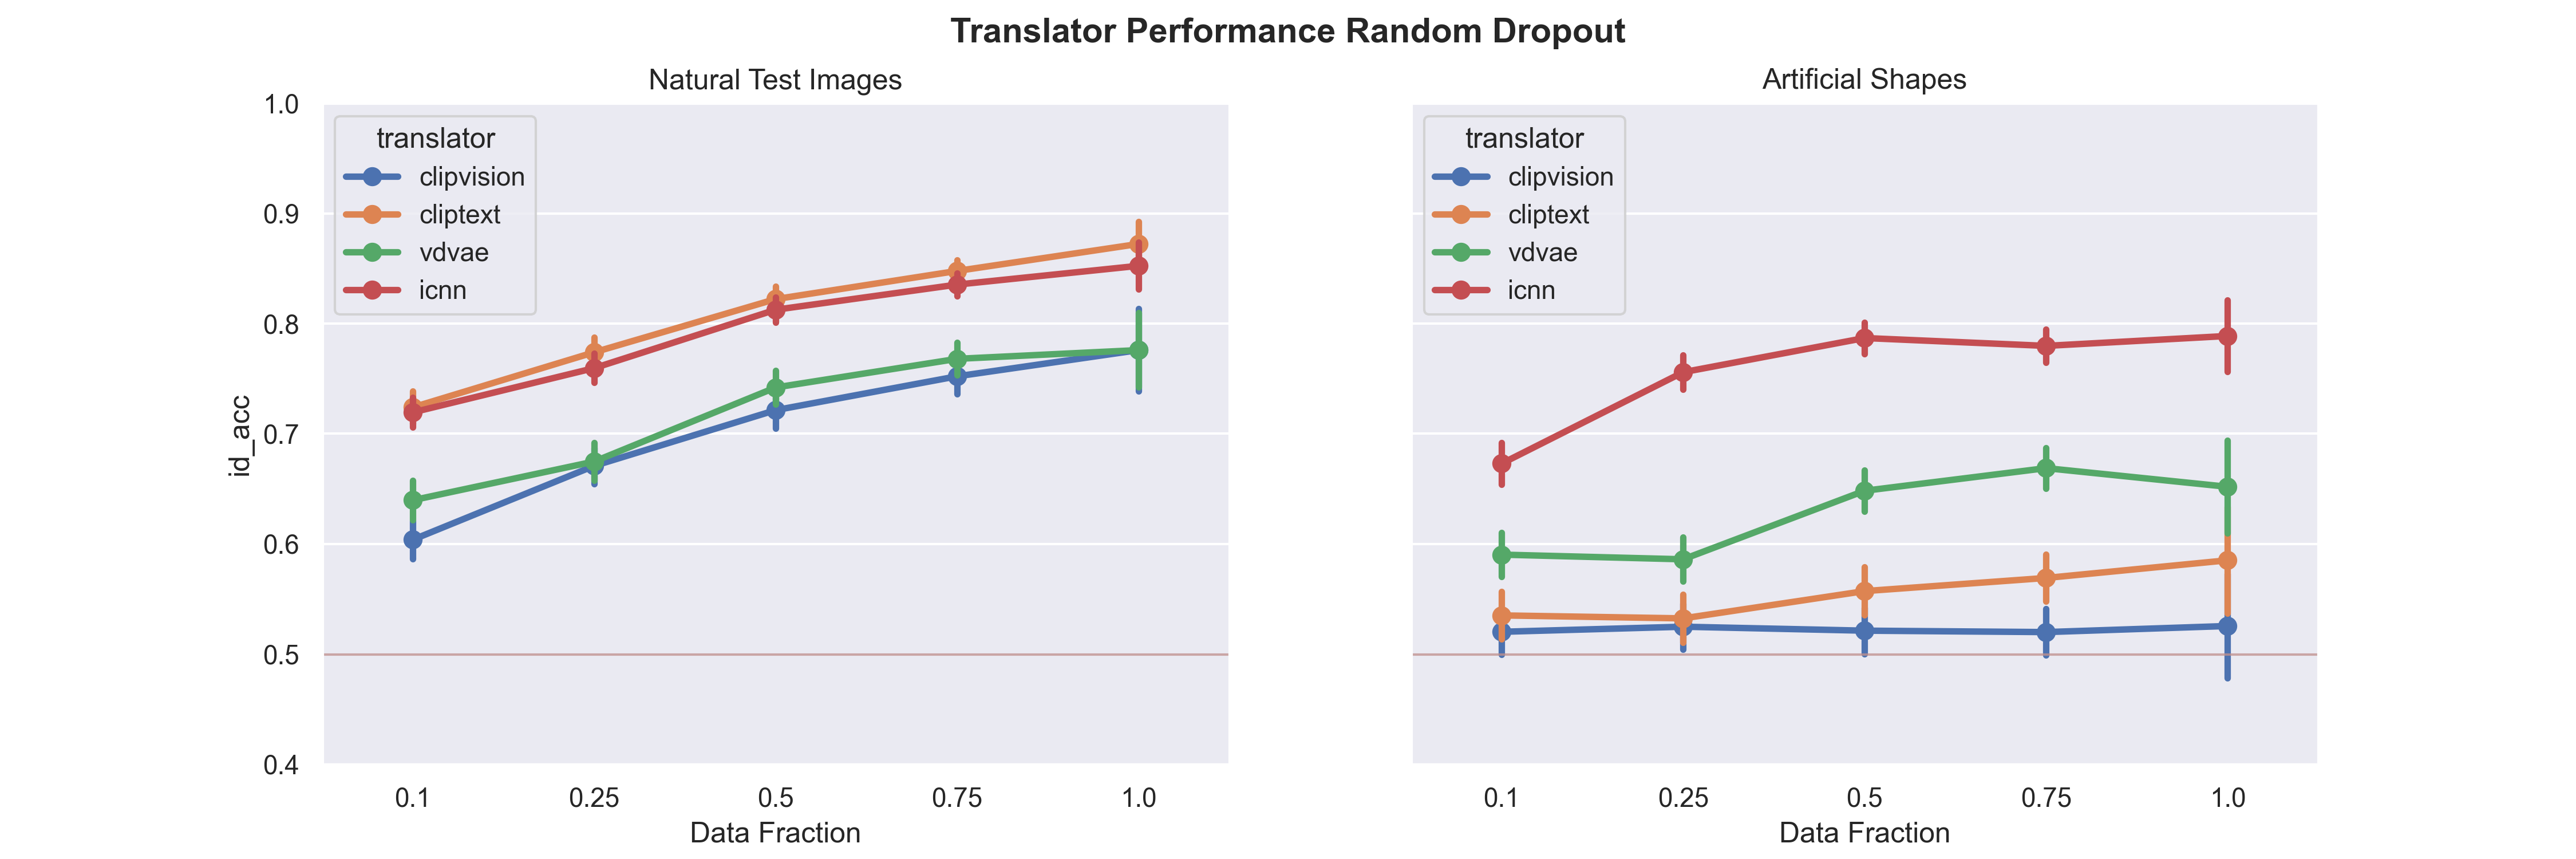
\includegraphics[width=1\textwidth]{plots/dropout_random_translator.png}
    \caption{A nice image}\label{fig:dropout_random_translator}
\end{figure}

% 2. Reconstruction Random Quant Plot test/art
\begin{figure}[ht]
    \centering
    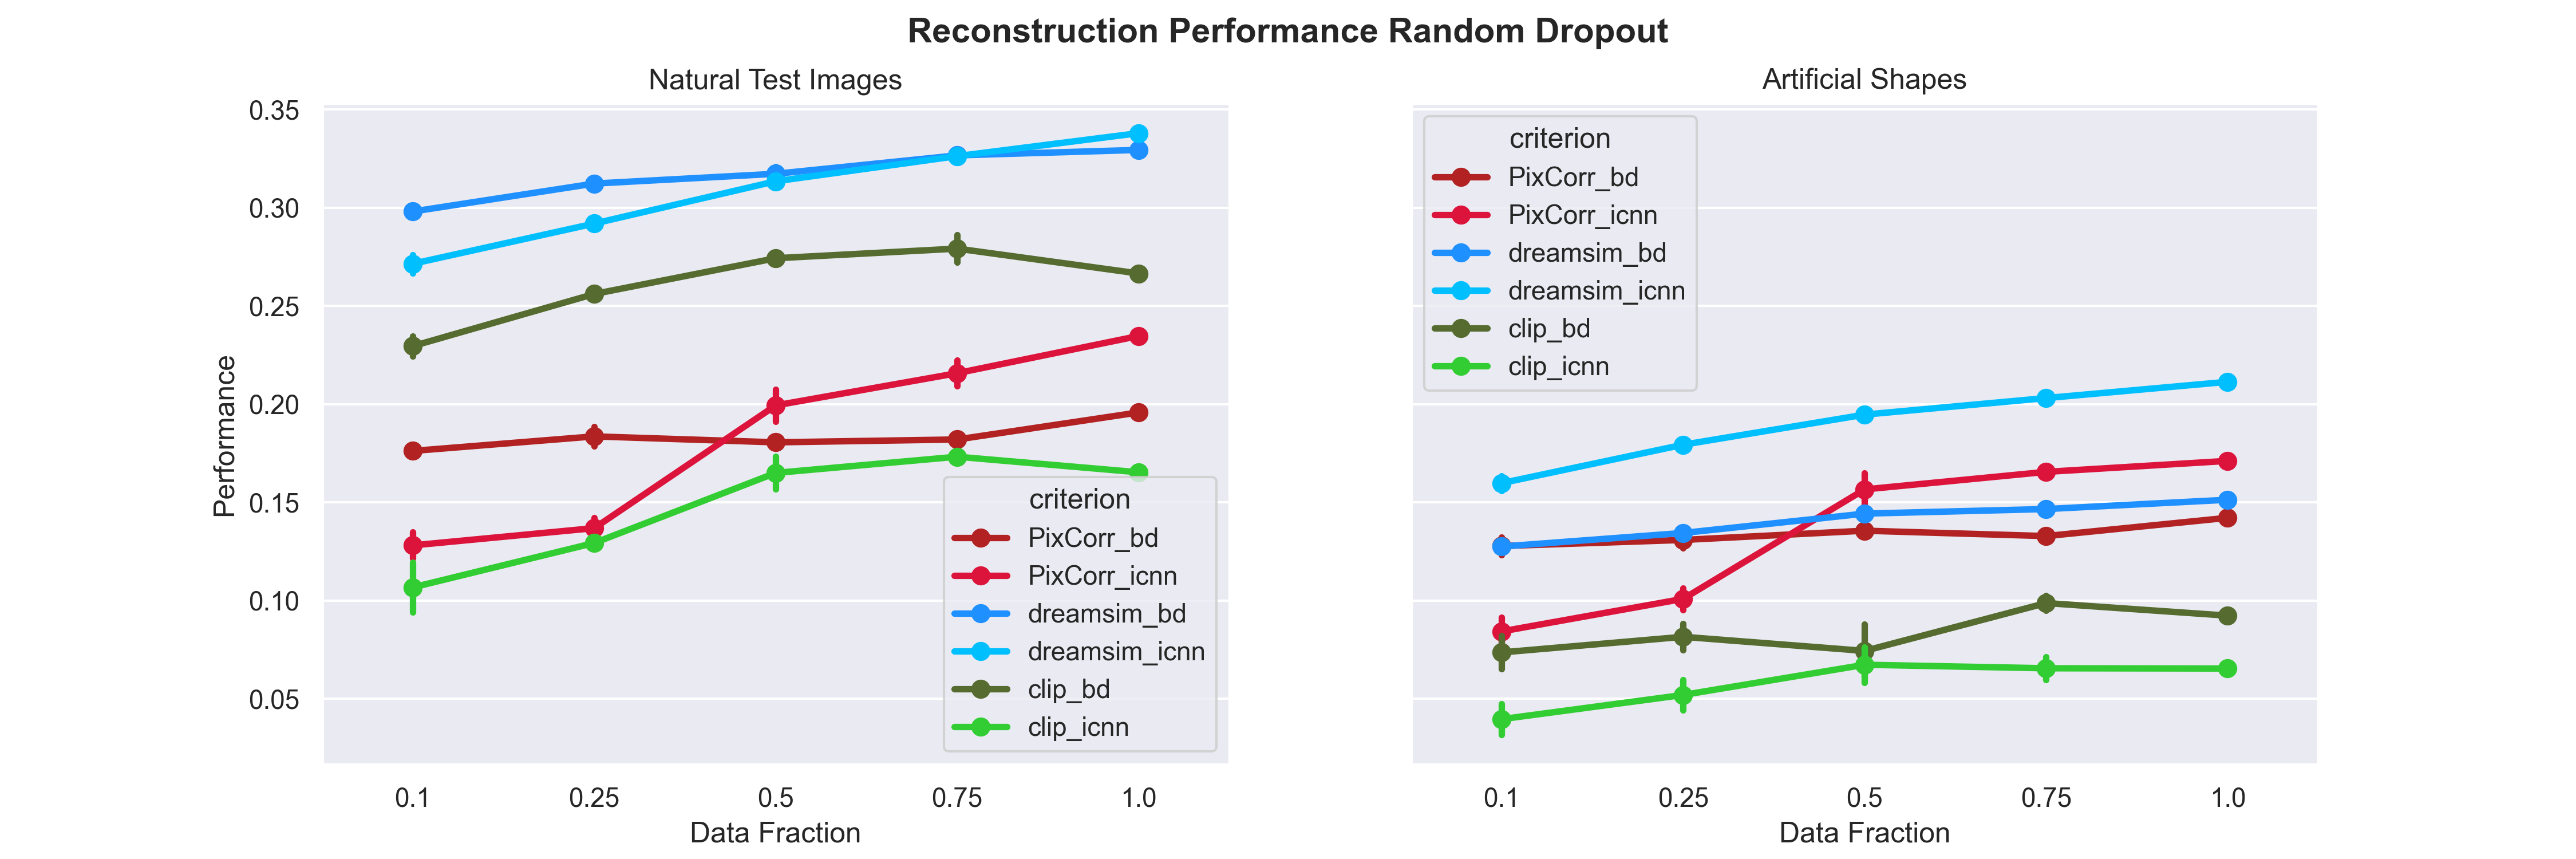
\includegraphics[width=1\textwidth]{plots/dropout_random_reconstruction.png}
    \caption{A nice image}\label{fig:dropout_random_reconstruction}
\end{figure}

The performance of the translator is shown in Figure~\ref{fig:dropout_random_translator} for both the natural test images and the artificial shapes. For the natural test images, the relationship between the number of training samples and performance is relatively similar for all the translators: the more training samples, the better. However, for the VDVAE and ICNN in particular, the performance curve for the translator flattens out at around 50\% training samples. The trend for the artificial shapes is somewhat different. The Clipvision translator does not seem to improve with an increasing number of training images, but is only just above the random level of 0.5. The Cliptext translator can show a performance above the random level from about 50\% of the training data set and then increases continuously. The VDVAE translator shows a slightly higher performance, but also saturates at about 50\% of the training data set. The same pattern is shown by the ICNN, whose performance is the best, but also does not improve from about 50\% of the training data set. 

The quantitative performance of the reconstruction algorithms is shown in Figure~\ref{fig:dropout_random_reconstruction} for both the natural test images and the artificial images. The individual metrics are shown in similar colours for Brain Diffuser and ICNN (ICNN is slightly lighter than Brain Diffuser). The PixelCorrelation shows a similar picture for both algorithms for the natural test images and the artificial shapes: While the ICNN benefits from more training samples, with the step from 25\% to 50\% of the training data set being particularly significant, the brain-diffuser shows only a very small increase in performance with increasing number of training samples. The Dreamsim similarity increases continuously with a larger number of training samples. In particular, the ICNN benefits from a larger number of training samples. The Clip-Accuracy shows that for the natural test images the performance also saturates at about 50\% of the training samples, and for the artificial shapes it is difficult to report an increase in performance.

% 3. Reconstruction Random Qual Plot test

\begin{figure}[ht]
    \centering
    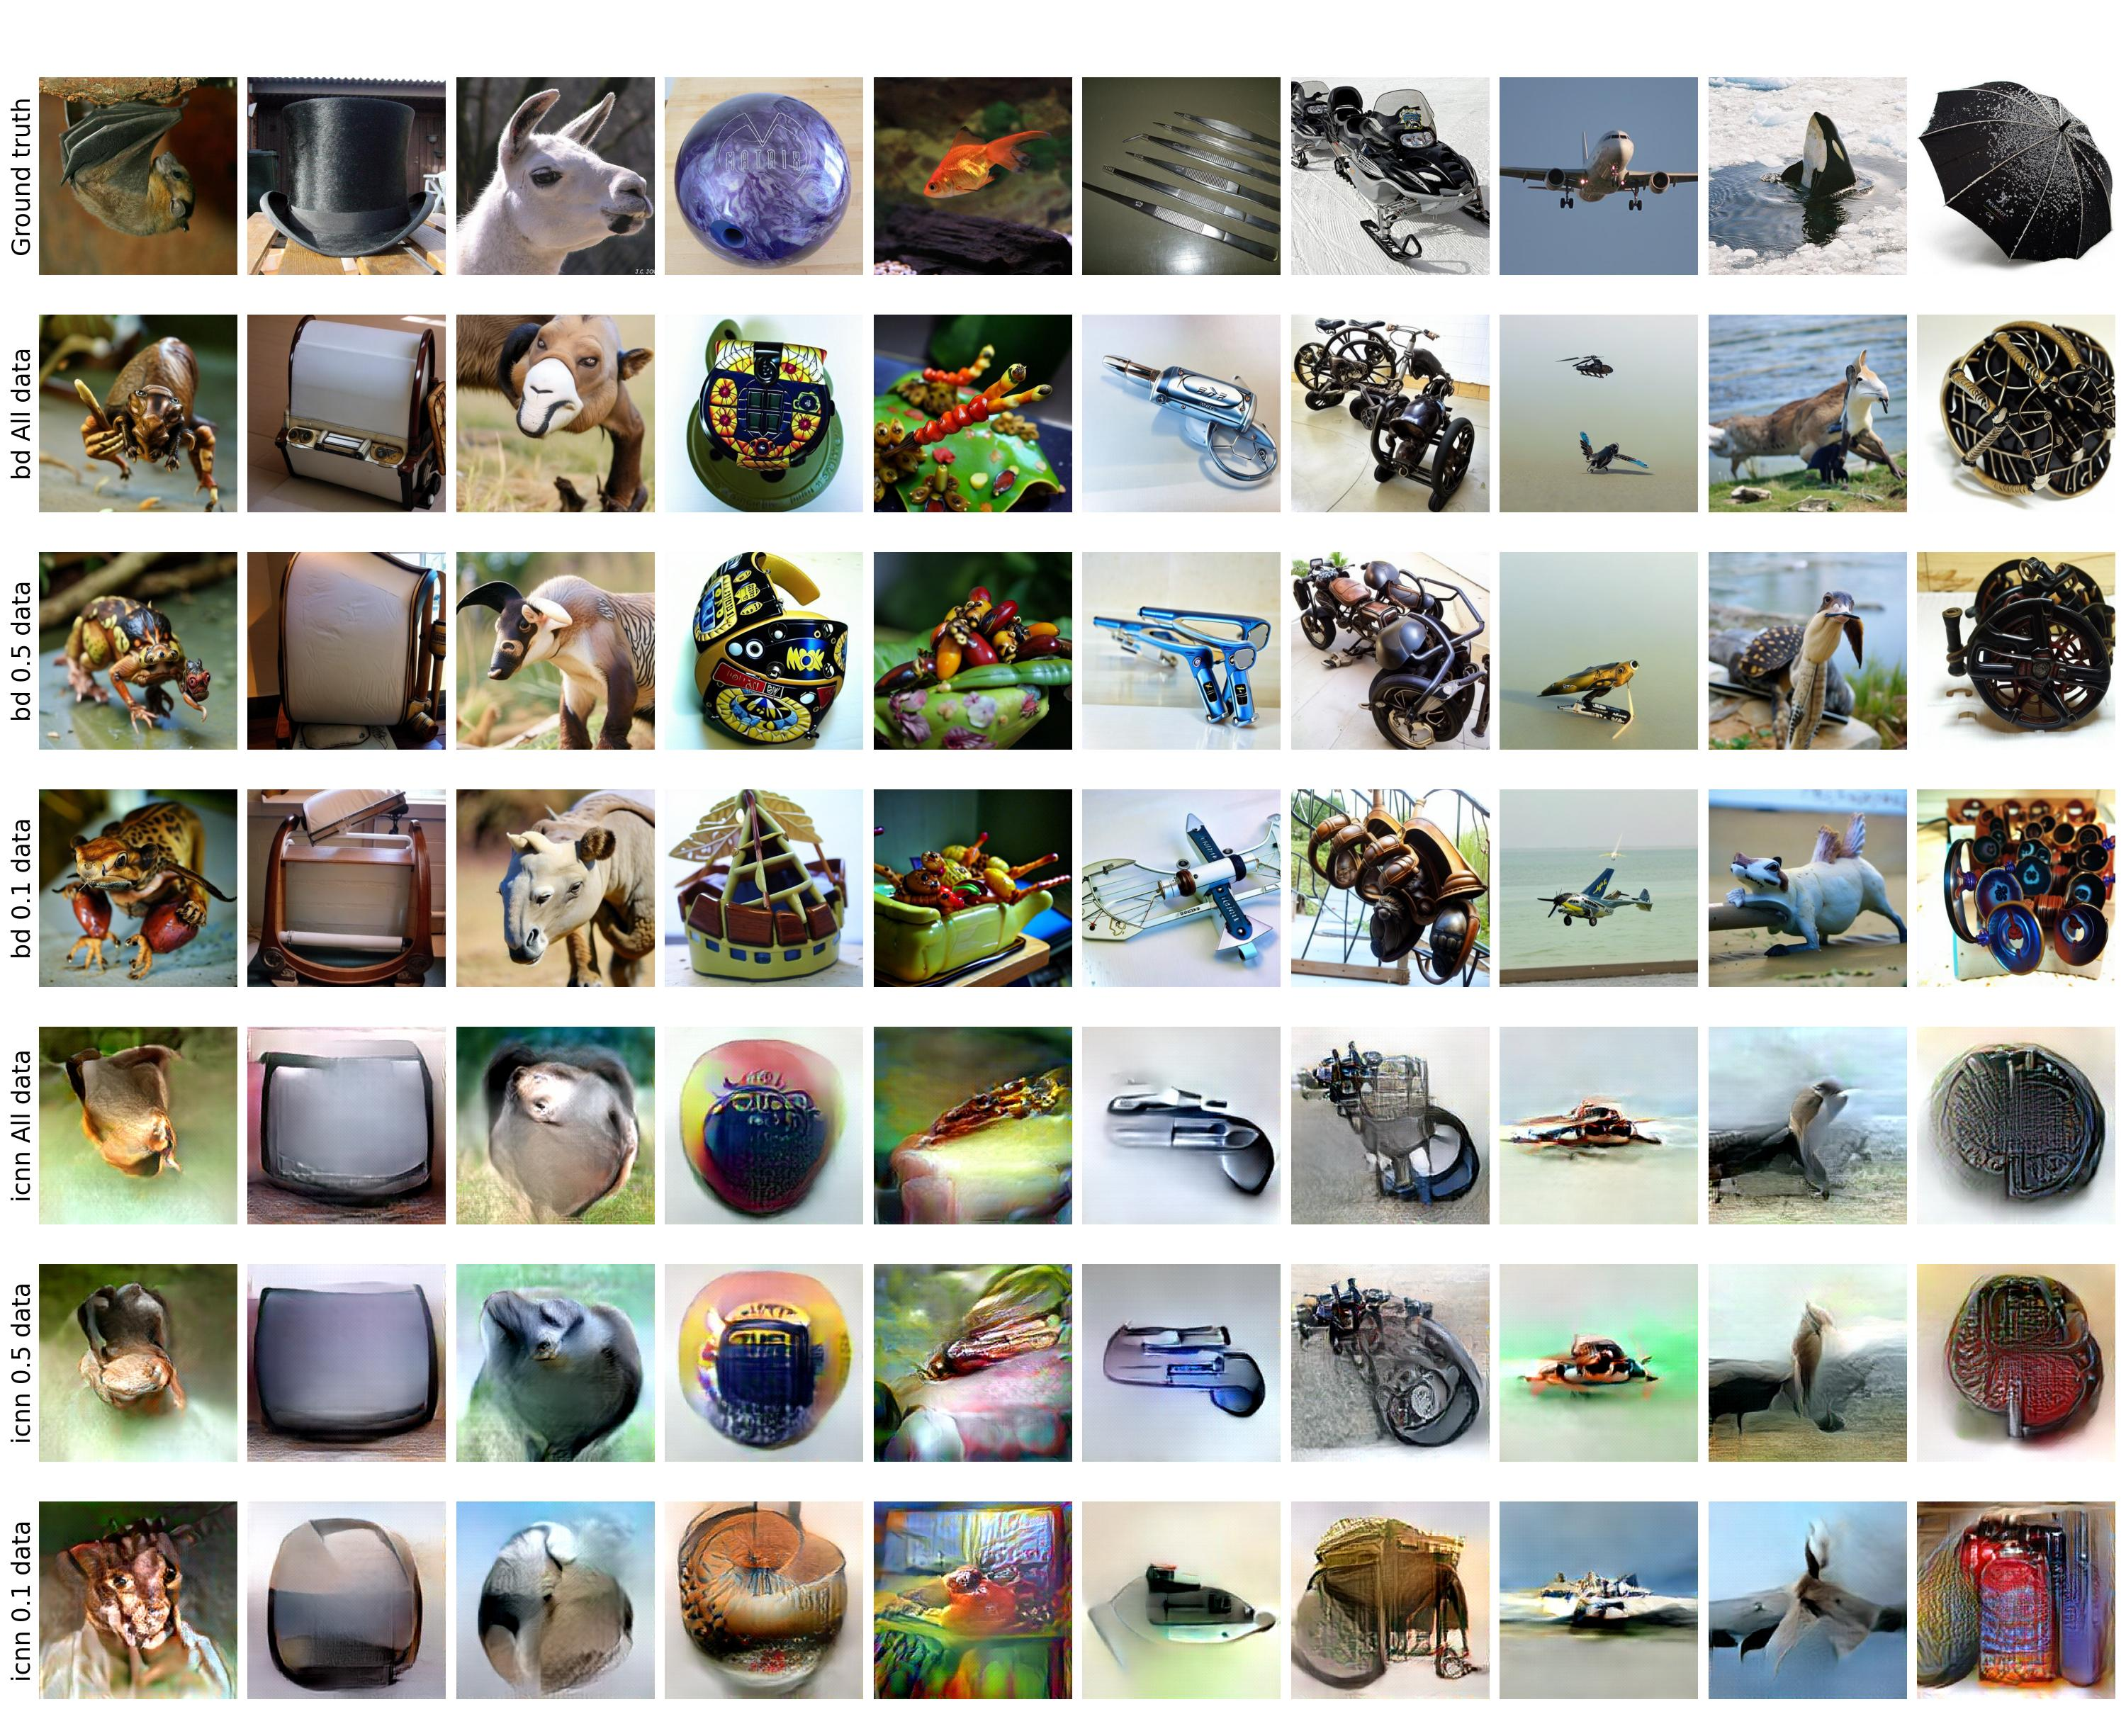
\includegraphics[width=1\textwidth]{plots/dropout_qual_random_test.JPEG}
    \caption{A nice image}\label{fig:dropout_qual_random_test}
\end{figure}

% 3.5 Reconstruction Random Qual Plot art
\begin{figure}[ht]
    \centering
    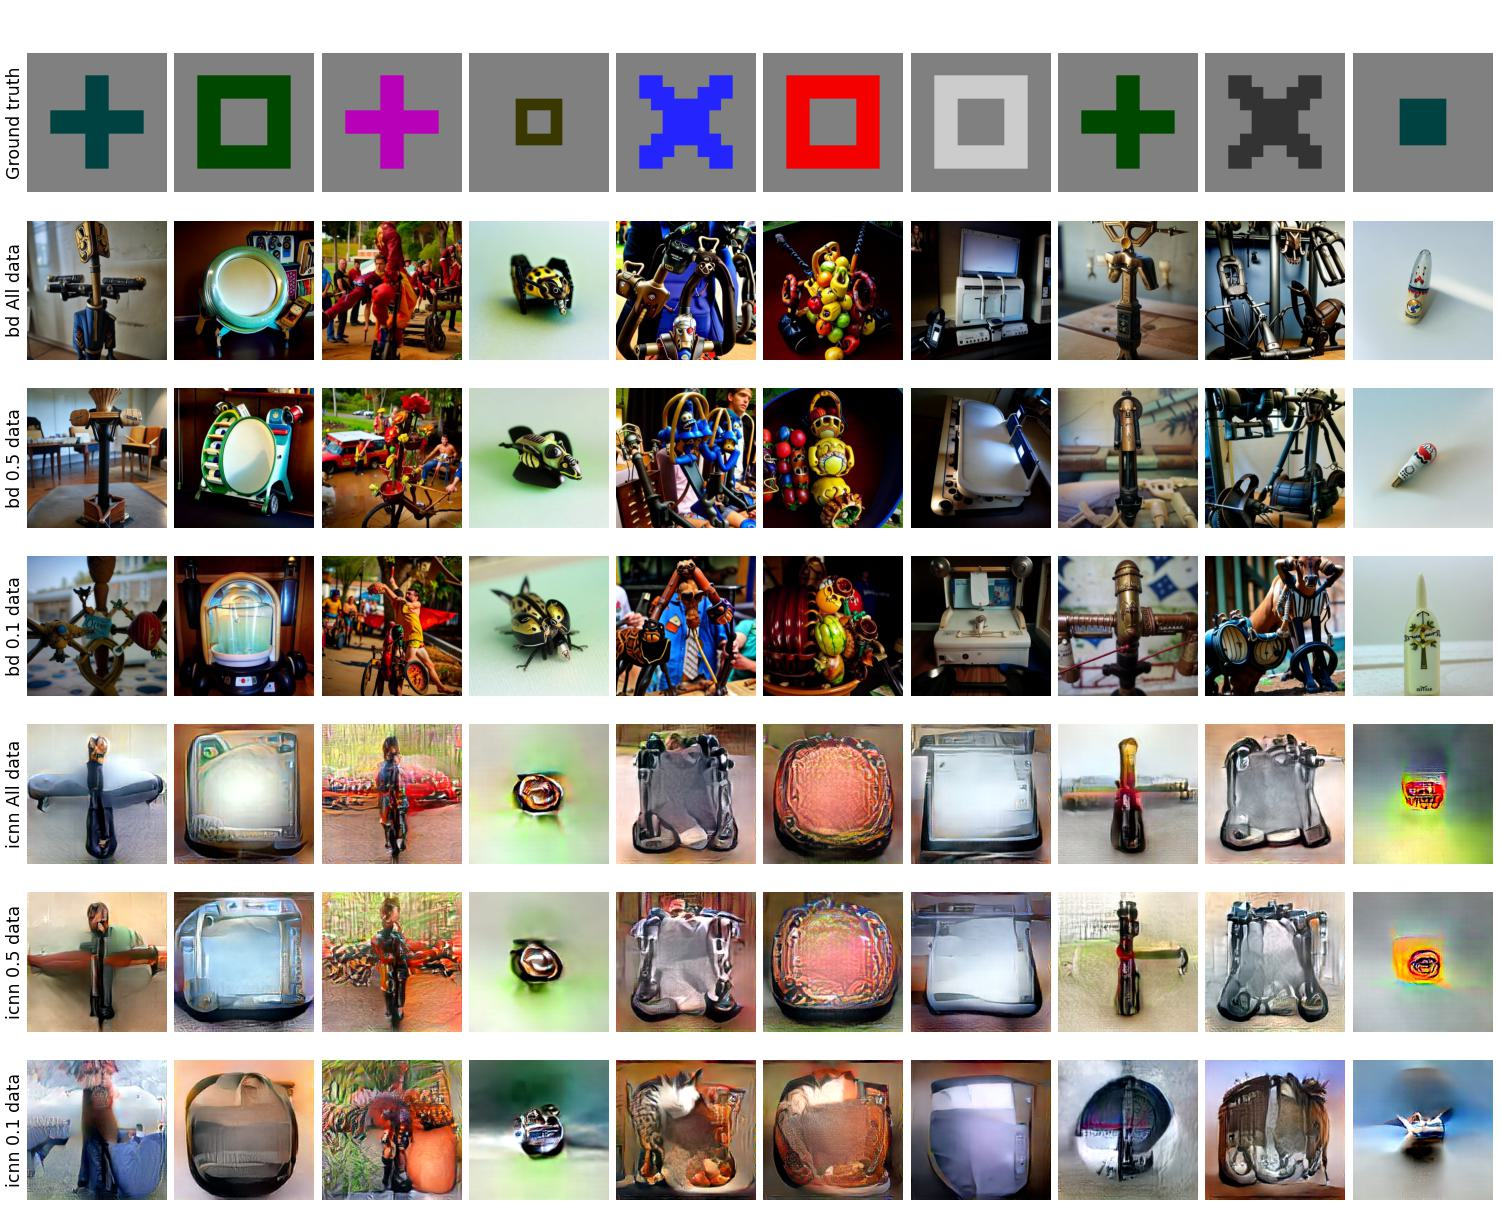
\includegraphics[width=1\textwidth]{plots/dropout_qual_random_art.JPEG}
    \caption{A nice image}\label{fig:dropout_qual_random_art}
\end{figure}

The qualitative performance of the reconstructions with different training set sizes can be seen in Figure~\ref{fig:dropout_qual_random_test} for the natural test images and in Figure~\ref{fig:dropout_qual_random_art} for the artificial shapes. It can be seen that even with only 10\% of the training images, distinctive features of the images can be reconstructed. However, it can also be seen that the quality of the reconstructions improves as the amount of training data increases. For example, the Brain Diffuser is not yet able to correctly classify the snowmobile as a vehicle with a small amount of training data, or the outlines of the goldfish are not yet nearly correct with the ICNN.\@ Interestingly, the reconstruction of the brain diffuser's aircraft is better with a small number of training samples than with the full data set. This is probably because the VDVAE, which produced artefacts for this image, still works with the small number of training samples. For the artificial shapes, there is a visible improvement in the quality of the reconstruction, especially for the ICNN, as the number of training samples increases. This goes along with the quantitative results.

In summary, it can be said that the performance in decoding and reconstruction can usually be significantly improved with an increasing number of training samples. In our example, many effects become visible in the step between 25\% and 50\% of the training data set, and in some cases the performance starts to saturate from this point on. For the following experiments, therefore, the data set should not contain more than 50\% of the training samples, in order to still have potential for performance improvement. At the same time, the training data set should not be smaller than 25\%, otherwise the decoding may not work well enough for testing.

\subsubsection{Diversity based Data-Subsampling}

For this work, the data should be subsampled as diversely as possible in order to produce a reduced dataset that can beat a randomly subsampled dataset in terms of decoding and reconstruction performance. In this work, a multi-step subsampling procedure is chosen: First, all training images are transformed into a latent feature space (within this feature space, an attempt is made to maximise diversity). Then, the nonlinear dimension reduction algorithm UMAP\cite{mcinnesUMAPUniformManifold2018} is used to reduce the dimensionality of the training images embedded in the feature space to two dimensions. The data in the UMAP space is then divided into $k$ clusters using k-means\cite{1056489} clustering (where $k$ is the number of images to be subsampled). For each of the $k$ clusters, the centroid of all $n$ images in that cluster is determined. Finally, for each cluster, the image with the smallest Euclidean distance to the centroid is selected. Using this procedure, $k$ images can be subsampled, where $k$ is arbitrary but must be less than the total number of training images. However, it should be clear that $k$ clusters cannot reasonably be found in the selected feature space; for example, if $k$ is selected very high (about 50\% of the dataset), only 2 images would be present in each cluster. To ensure that the subsampling algorithm can produce a meaningful subselection of the training set, k should be chosen as small as possible. Given the results of the random subselection baseline in the previous chapter, $k$ is set to 25\% (i.e. 300) of the images in the training set. 

% 4 UMAP
\begin{figure}[ht]
    \centering
    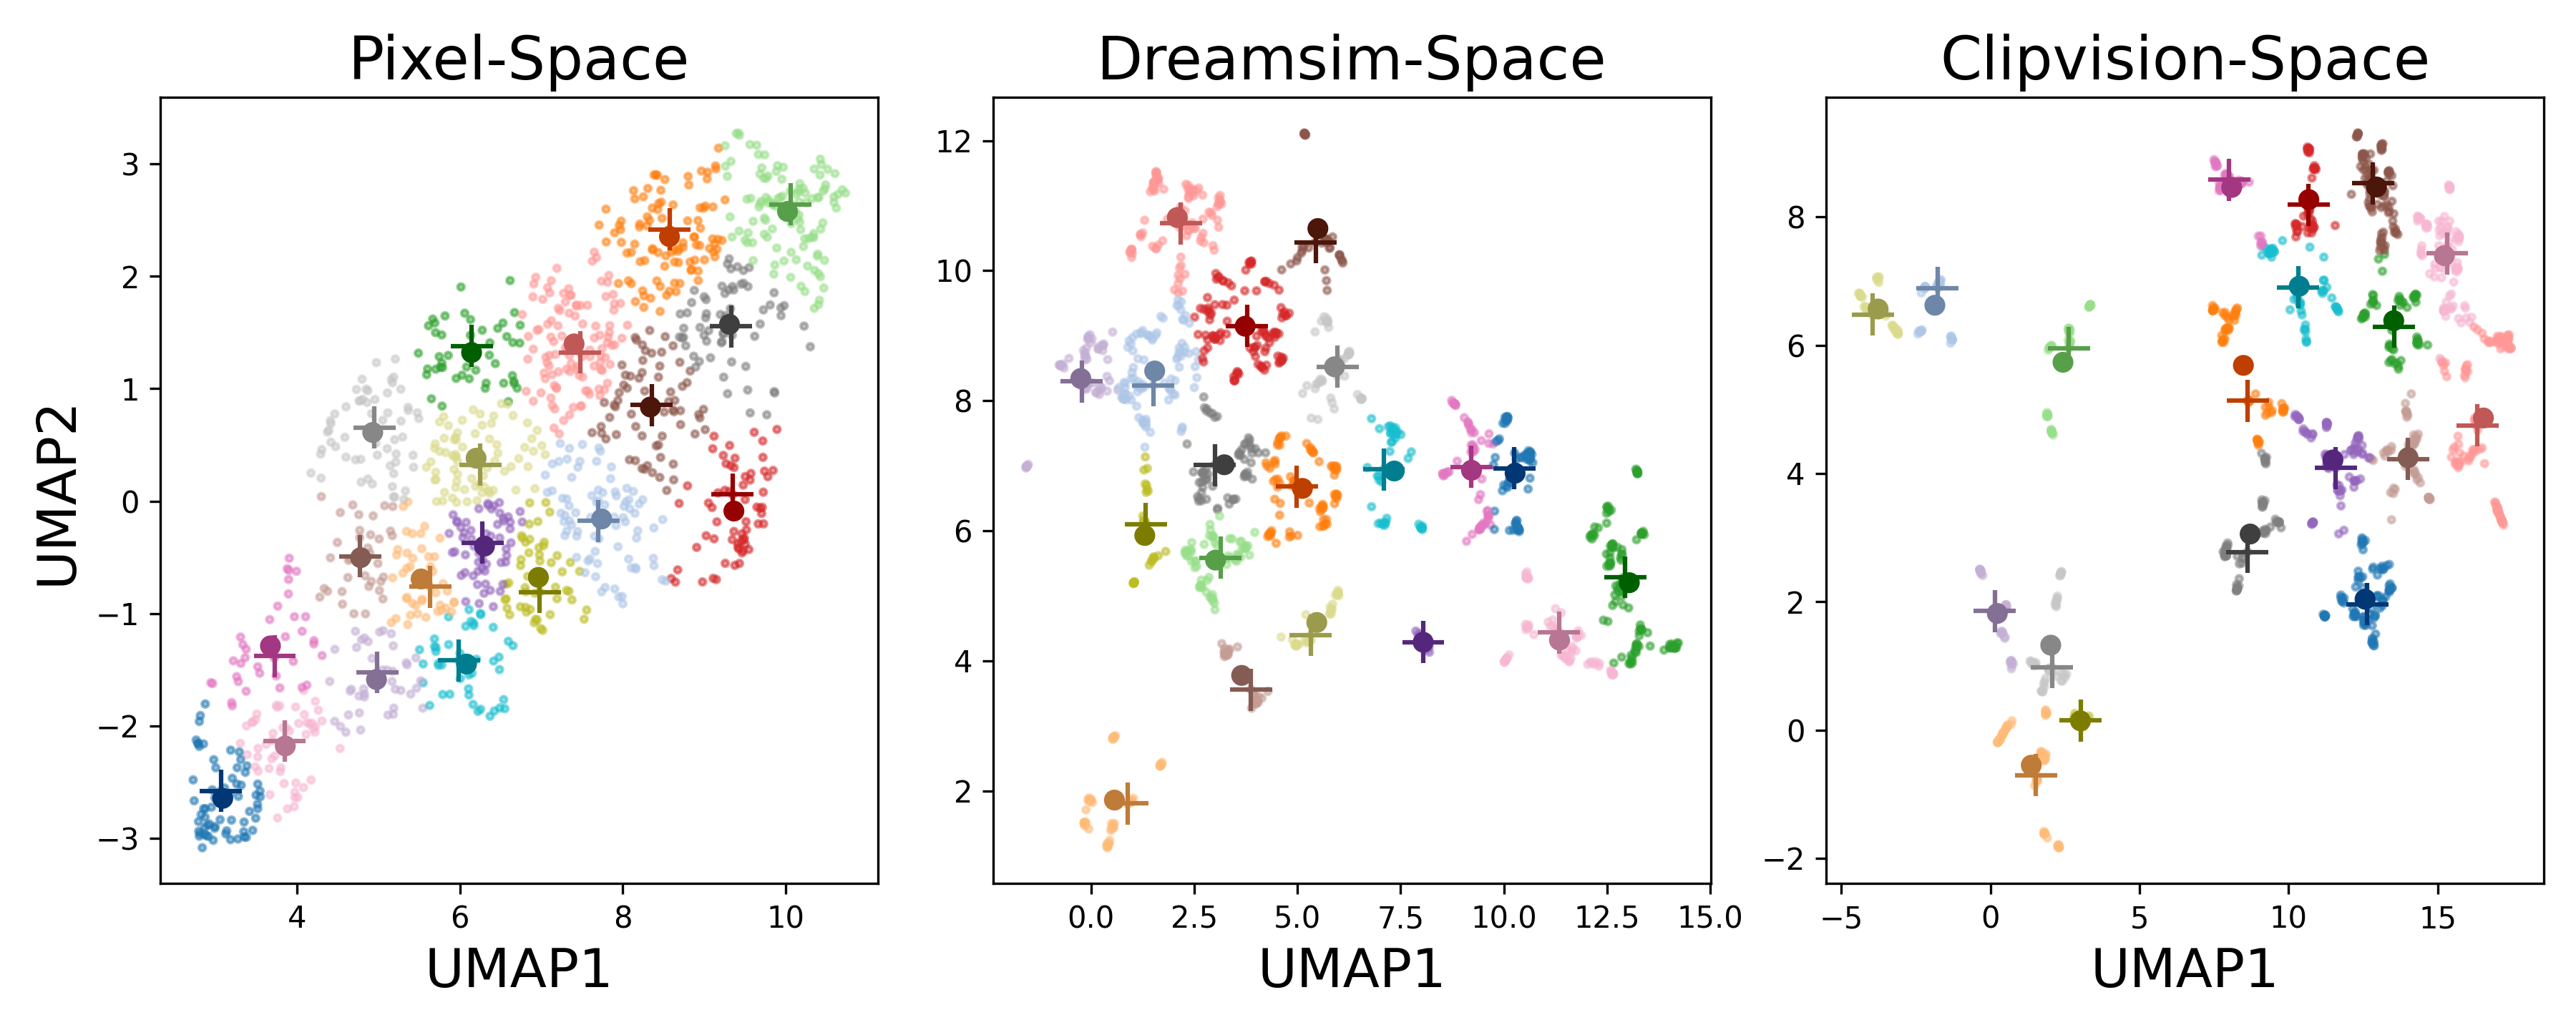
\includegraphics[width=0.9\textwidth]{plots/dropout_umap.png}
    \caption{UMAP + k-means of Pixel-Space, Dreamsim and Clipvision Space}\label{fig:dropout_umap}
\end{figure}




The feature space in which the training images are initially embedded is freely selectable. To follow the logic of the evaluation criteria, a low-level, a mid-level and a high-level representation are chosen. For the low-level representation, the images (resized to 200$\times$200 pixels) are simply concatenated into a one-dimensional vector, so that the subsequent UMAP algorithm can only reduce the dimensions at the pixel level (this procedure was successfully applied by the authors of UMAP to the MNIST dataset). For the mid-level representation, the training images are embedded with Dreamsim\cite{fuDreamSimLearningNew2023}, for the high-level representation, the training images are embedded in clip-space using clipvision\cite{radfordLearningTransferableVisual2021}. Thus, all images are transformed into one-dimensional vectors whose dimensionality is reduced using UMAP and clustered using k-means. 
The results of the selection process are shown as an example in Figure~\ref{fig:dropout_umap}. In the plots, the number of clusters has been set to $k=20$ for visualisation purposes. Each point in the plot represents a slice of the training data set in UMAP space. The clusters are coloured differently. The centroid of each cluster is shown as a circle and the image closest to the centroid is marked with a cross. In Dreamsim and Clipvision space, the different clusters are already clearly separated from each other in the two dimensions of UMAP, while the result in pixel space has divided the images comparatively homogeneously, which may indicate that the UMAP dimension reduction has not worked optimally (this can probably be explained by the high number of dimensions in pixel space 200$\times$200$\times$3 colour channels = 120000). 
Subsamples with 25\% (300 images) of the training data set were extracted for each of the feature spaces using the method described above. Figure~\ref{fig:dropout_similarity_plot} shows the most similar image in the reduced dataset for each feature space for ten images from the input dataset (left column). This shows the differences in sampling in the three feature spaces: in the Dreamsim and Clipvision spaces, the images are relatively similar to the original. However, the differences between the mid-level and high-level similarities become clear. For example, in the case of the revolver in the first image, Dreamsim selects a gun that is relatively similar in the image, but is the wrong type. Clipvision selects an image that is a better semantic match because it also shows a revolver, even though the remaining visual similarity is lower (colour of the gun, partially covered by a hand). This difference between clipvsion and Dreamsim can also be seen in other images. In pixel space, however, the subjective similarity between the original and the sample is lower. In the third image, for example, the original shows an ear with white headphones, while the most similar image in pixel space is a goose with a long white neck. The low-level match between the images is presumably an elongated white object in the middle. 

% 5 Umap Subselection Similarity from low_level_clustering.py
\begin{figure}[ht]
  \centering
  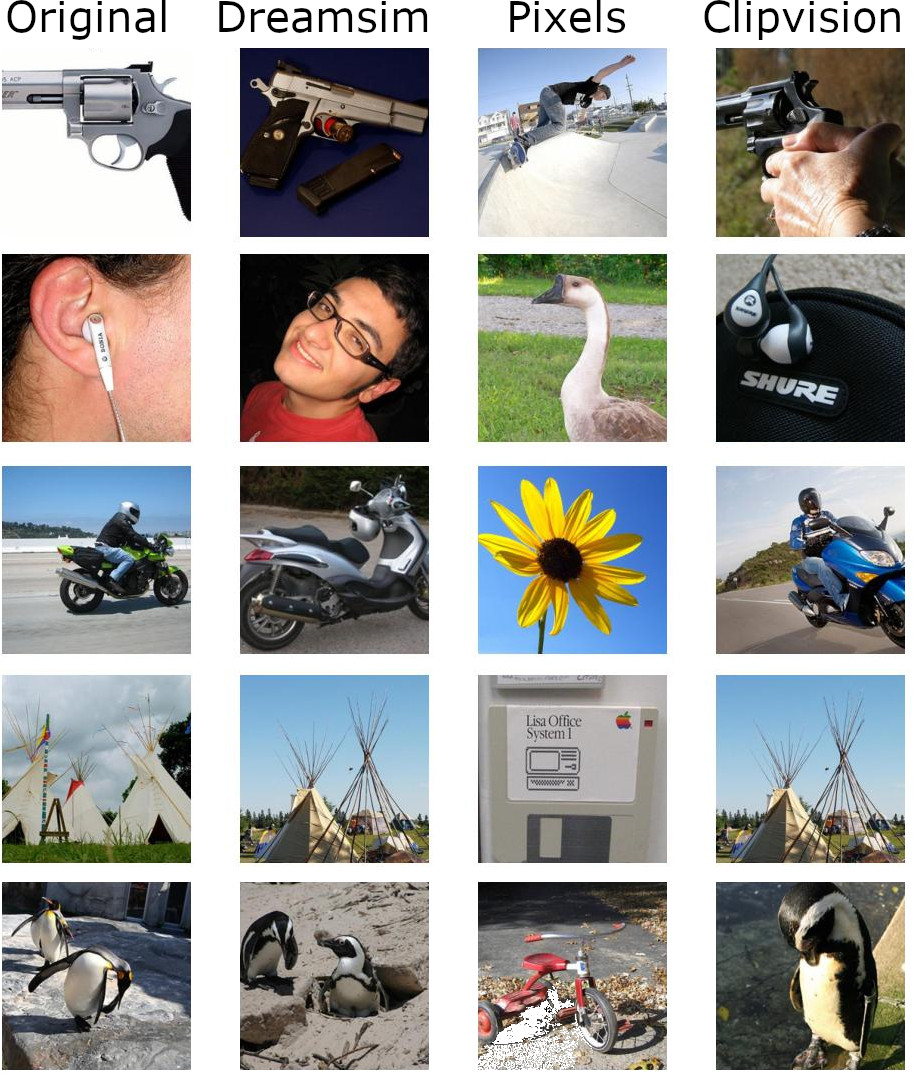
\includegraphics[width=0.6\textwidth]{plots/dropout_similarity_plot.JPEG}
  \caption{Most similar image to original in multiple subspaces}\label{fig:dropout_similarity_plot}
\end{figure}

In order to ensure that the subselection has indeed increased the diversity in the feature space, it is validated quantitatively. For this purpose, a new metric is defined, the average minimum distance to all training samples (avg\_min\_dist). It is defined as follows

\[
\text{avg\_min\_dist}
= \frac{1}{n_{\text{all}}}
  \sum_{i=1}^{n_{\text{all}}}
    \min_{1 \le j \le n_{\text{sub}}}
      \Bigl\lVert f(\mathbf{x}_i) - f(\mathbf{y}_j) \Bigr\rVert
\]

\[
\begin{aligned}
n_{\text{all}} &:=
  \text{number of images in the full set}, \\
n_{\text{sub}} &:=
  \text{number of images in the subsample}, \\
\mathbf{x}_i &:=
  \text{the $i$-th image in the full training dataset}, \\
\mathbf{y}_j &:=
  \text{the $j$-th image in the subsample}, \\
f &:=
  \text{embedding function from image feature space (Pixels, clipvision, dreamsim)}, \\
\|\cdot\| &:=
  \text{the Euclidean (L2) norm}.
\end{aligned}
\]

The avg\_min\_dist measures how close on average each image in the full training dataset  (embedded in the respective feature space) is to the next possible image in the subsample. If the subsample adequately represents the feature space, then for each input image there would be a comparatively close candidate in the subsample. The avg\_min\_dist was computed for all three feature spaces and is shown in Figure~\ref{fig:dropout_avg_min_distance}. For each subspace, 30 different samples were taken and the avg\_min\_dist was calculated for each sample. The figure shows that in each feature space, the subsample created using the corresponding feature space has the lowest avg\_min\_dist. The result is most ambiguous for the avg\_min\_dist in the pixel feature space, but again the subsample created using the pixel space has the lowest avg\_min\_dist. The avg\_min\_dist for dreamsim and clipvision are always comparatively close, which makes sense since dreamsim is partly based on clipvision\cite{fuDreamSimLearningNew2023}. 

\begin{figure}[ht]
    \centering
    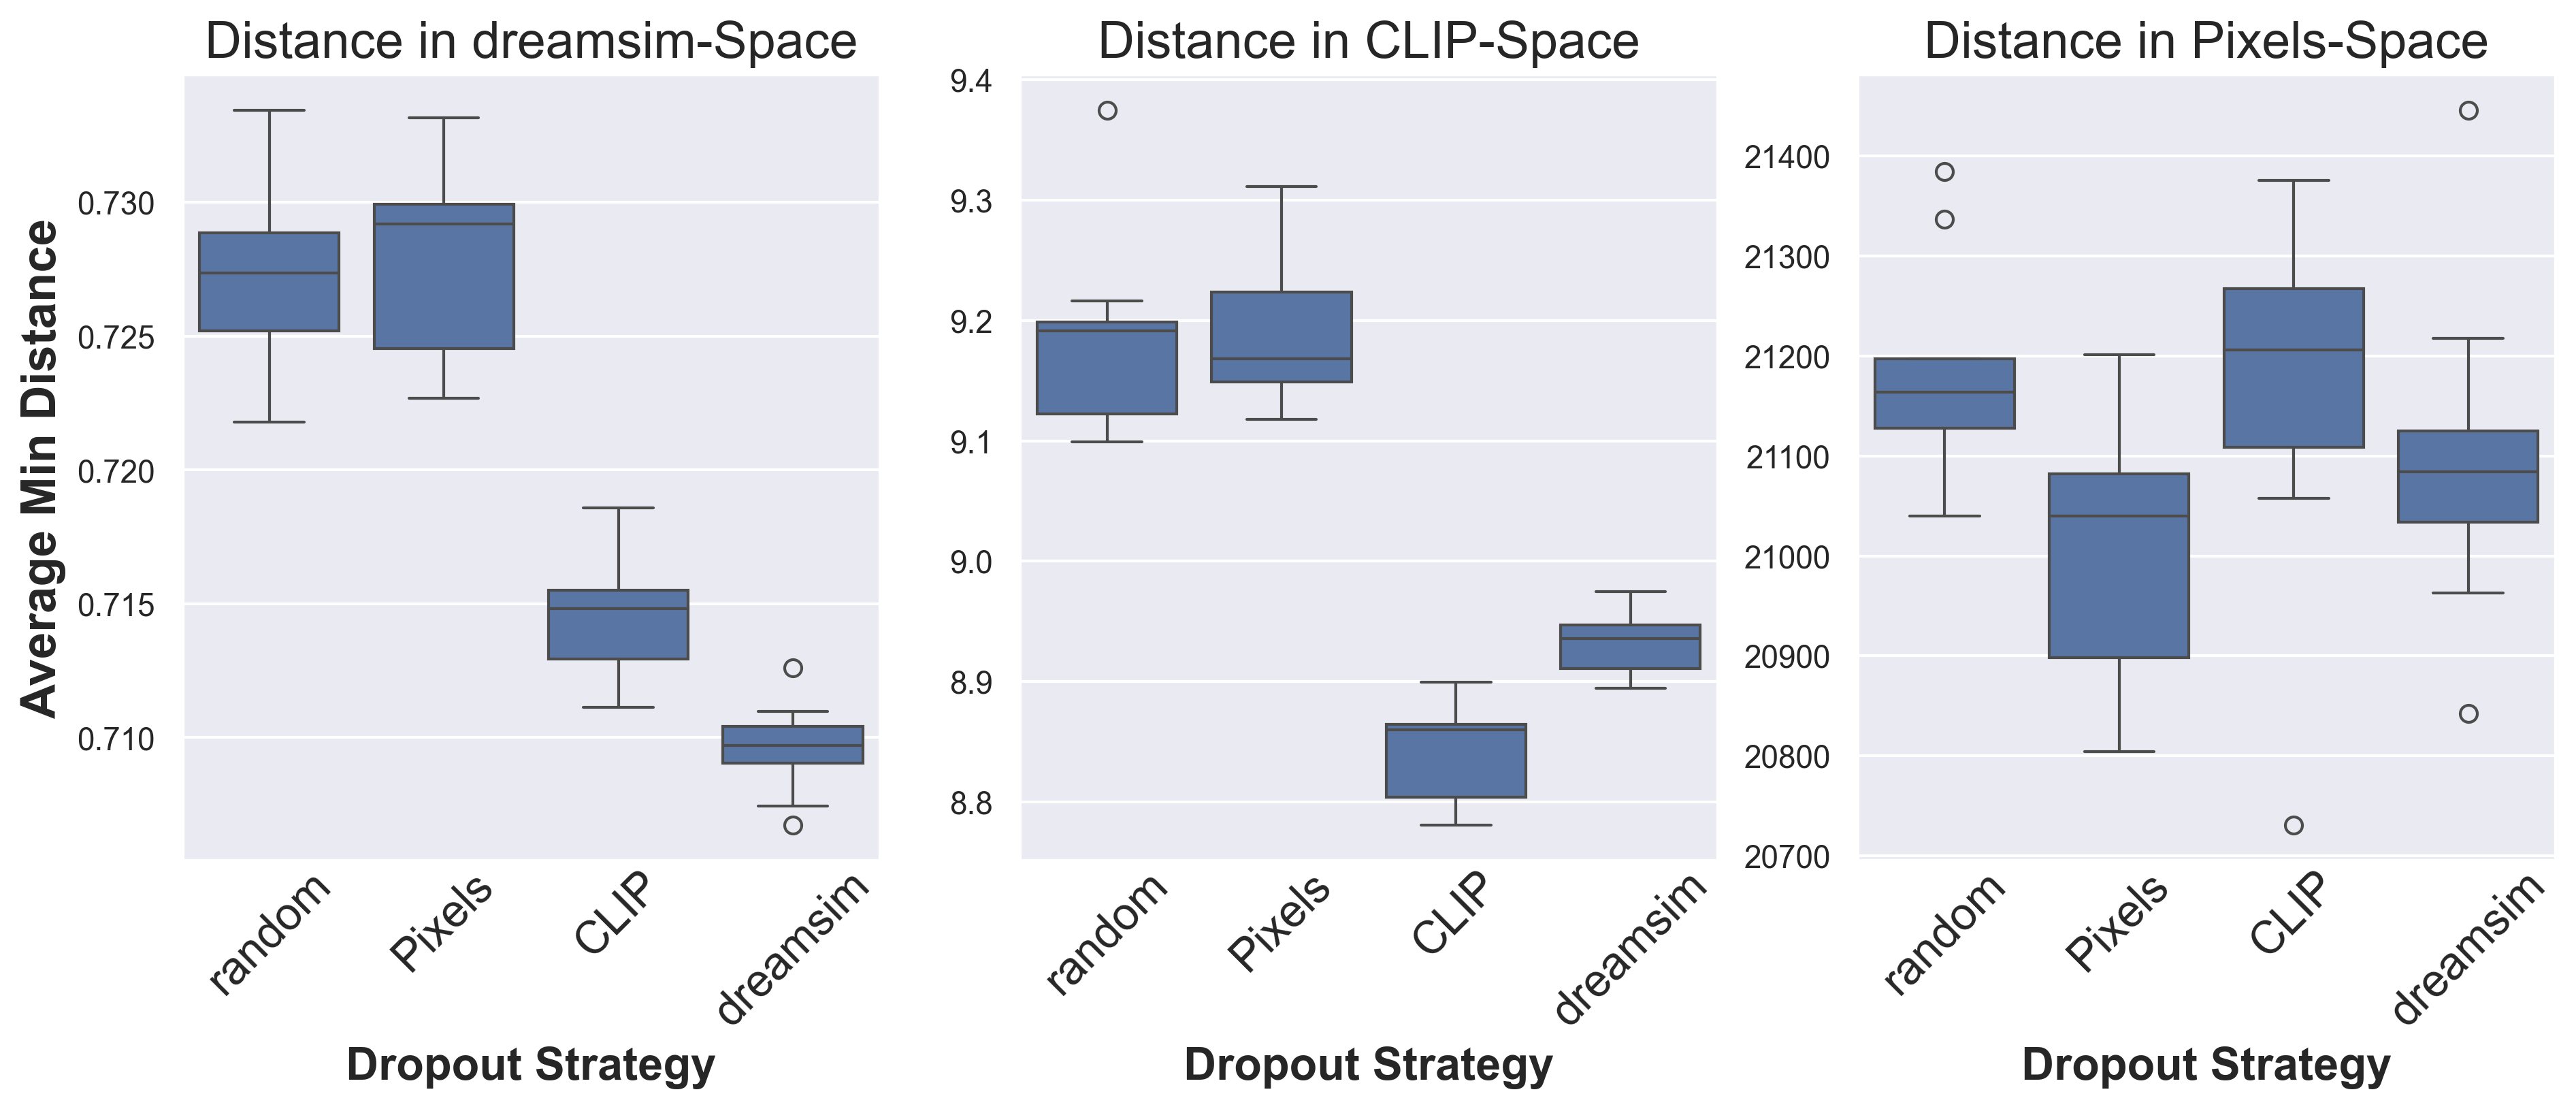
\includegraphics[width=1\textwidth]{plots/dropout_avg_min_distance.png}
    \caption{Avg-min-distance of subsample to All Training Images}\label{fig:dropout_avg_min_distance}
\end{figure}


In summary, the qualitative and quantitative review showed that the diversity-based subsampling method is successful in increasing the diversity in the respective subspace. For each feature space, the subsample with the lowest avg\_min\_dist in the validation (i.e.\ best representing the entire feature space) is used for further analysis.


\subsection{Results}
The three generated subspaces were used below to train the translator and reconstruct images for each of the five subjects. To provide an adequate baseline, the results of the three subspaces are each compared with a random subselection. 

\subsubsection{Decoding results}
The performance of the three trained translators of the brain diffuser and the VGG19 features of the ICNN algorithm is shown in Figure~\ref{fig:dropout_eval_translator_test} for the natural test images and in Figure~\ref{fig:dropout_eval_translator_art} for the artificial shapes. The results are shown for all four different dropout strategies (random subsample and samples based on the three feature spaces). For the natural test images, the performance of all subsamples is above the random probability of 0.5. However, for the three translators of the brain diffuser, there are no discernible differences in performance between the different dropout strategies. Only the ICNN translator shows that performance can be slightly improved with a targeted diversity-based subsampling strategy. However, in this case too, there is no significant difference between the three feature spaces.

% Now the Eval Results
% 7.1 Eval Translator test
\begin{figure}[ht]
  \centering
  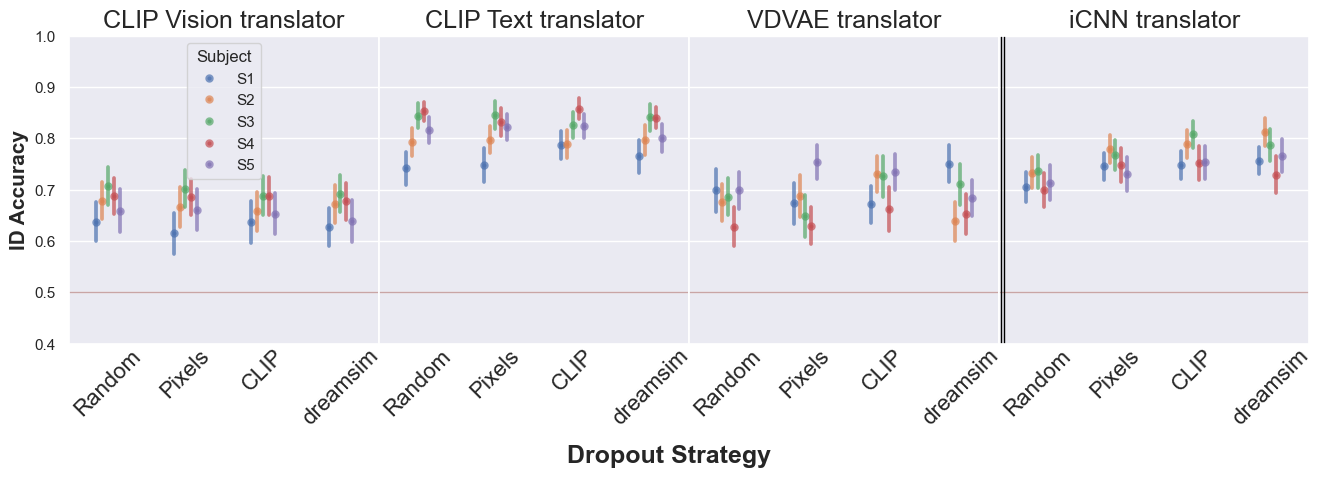
\includegraphics[width=1\textwidth]{plots/dropout_eval_translator_test.png}
  \caption{Translator performance (0.25 data fraction) for Natural Test Images}\label{fig:dropout_eval_translator_test}
\end{figure}

The artificial shapes in Figure~\ref{fig:dropout_eval_translator_art} show that the two clip translators are not able to significantly predict the features beyond random probability. This is independent of the subsampling space. The performance of the VDVAE translator is slightly better, with all subsamples tending to be better than the random probability. In particular, the performance of the low-level feature space pixel seems to have a slight advantage over the other subsampling strategies. For the ICNN translator, on the other hand, the effect of the natural test images seems to have been reversed; for the Pixel and Dreamsim feature spaces, the performance even looks slightly worse than with random subsampling. Within the clipvision feature space, the variance between the subjects is really high, thus the results cannot easily be interpreted.

\begin{figure}[ht]
  \centering
  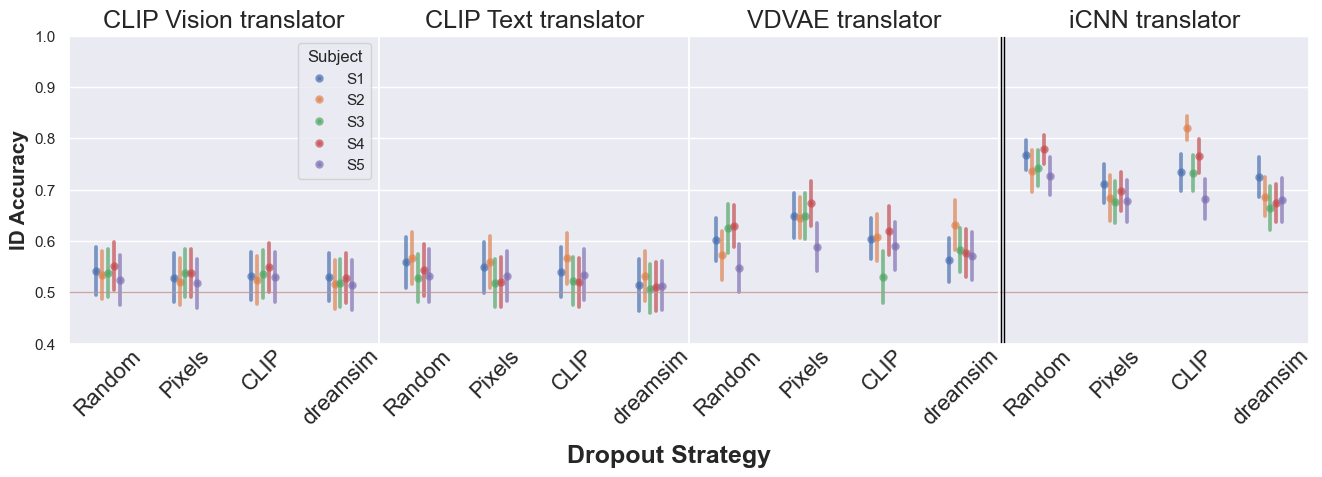
\includegraphics[width=1\textwidth]{plots/dropout_eval_translator_art.png}
  \caption{Translator performance (0.25 data fraction) for Artificial Shapes}\label{fig:dropout_eval_translator_art}
\end{figure}


\subsubsection{Reconstruction Results}

\begin{figure}[ht]
  \centering
  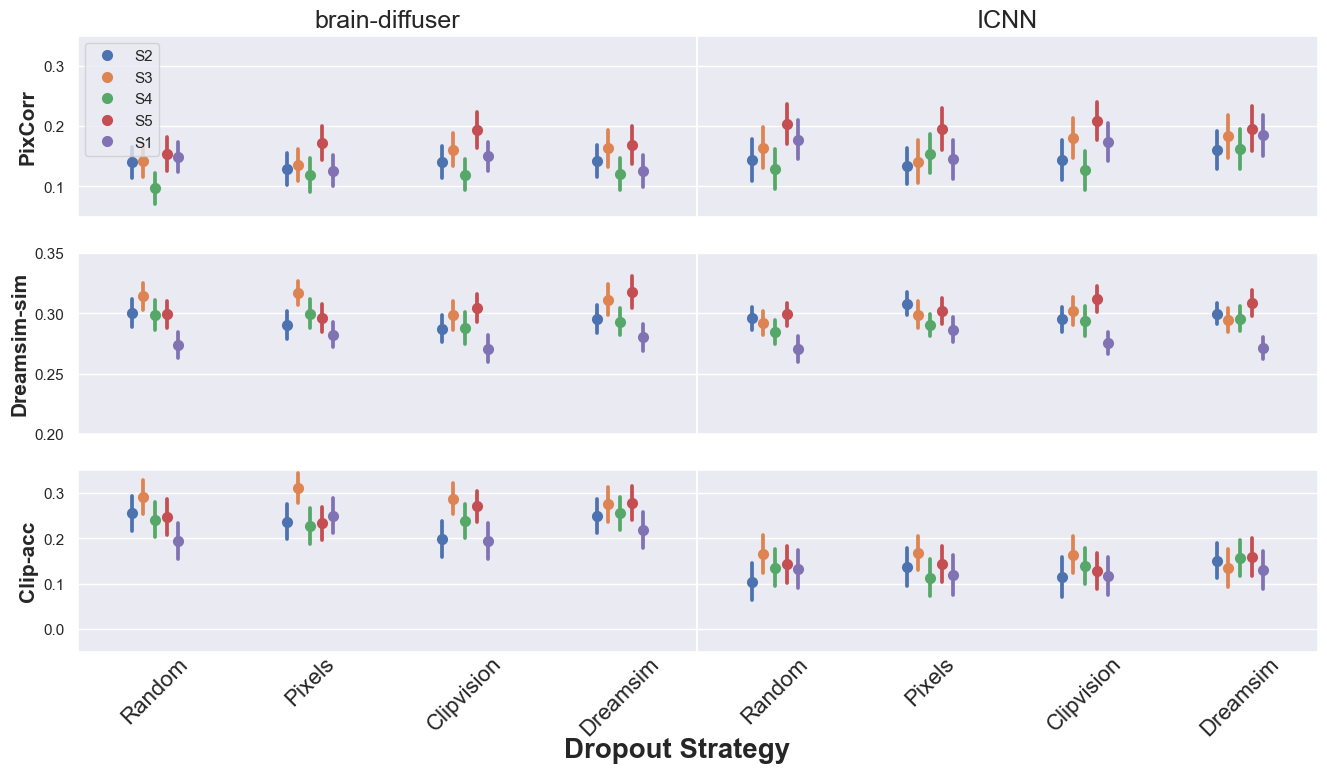
\includegraphics[width=1\textwidth]{plots/dropout_eval_reconstruction_test.png}
  \caption{Reconstruction Performance (0.25 data fraction) for Natural Test Images}\label{fig:dropout_eval_reconstruction_test}
\end{figure}

The quantitative results of the reconstructions using the four different subsamples are shown in Figure~\ref{fig:dropout_eval_reconstruction_test} for the natural test images and in Figure~\ref{fig:dropout_eval_reconstruction_art} for the artificial shapes. The three previously described criteria of PixelCorrelation, Dreamsim-similarity and Clip-Accuracy are specified for the Brain Diffuser and ICNN algorithms respectively. For the natural test images, there is no discernible difference between the random subselection and the three diversity-based subsamples for the Brain Diffuser in any of the three metrics. The results are similar for the ICNN. Although the translator performance was slightly improved beforehand, these effects seem to have only a partial and minor impact on the reconstruction performance. Only with the help of the Dreamsim-sim metric is there a slight increase in performance across all three feature spaces in contrast to the baseline. There are no differences between the feature spaces however.

\begin{figure}[ht]
  \centering
  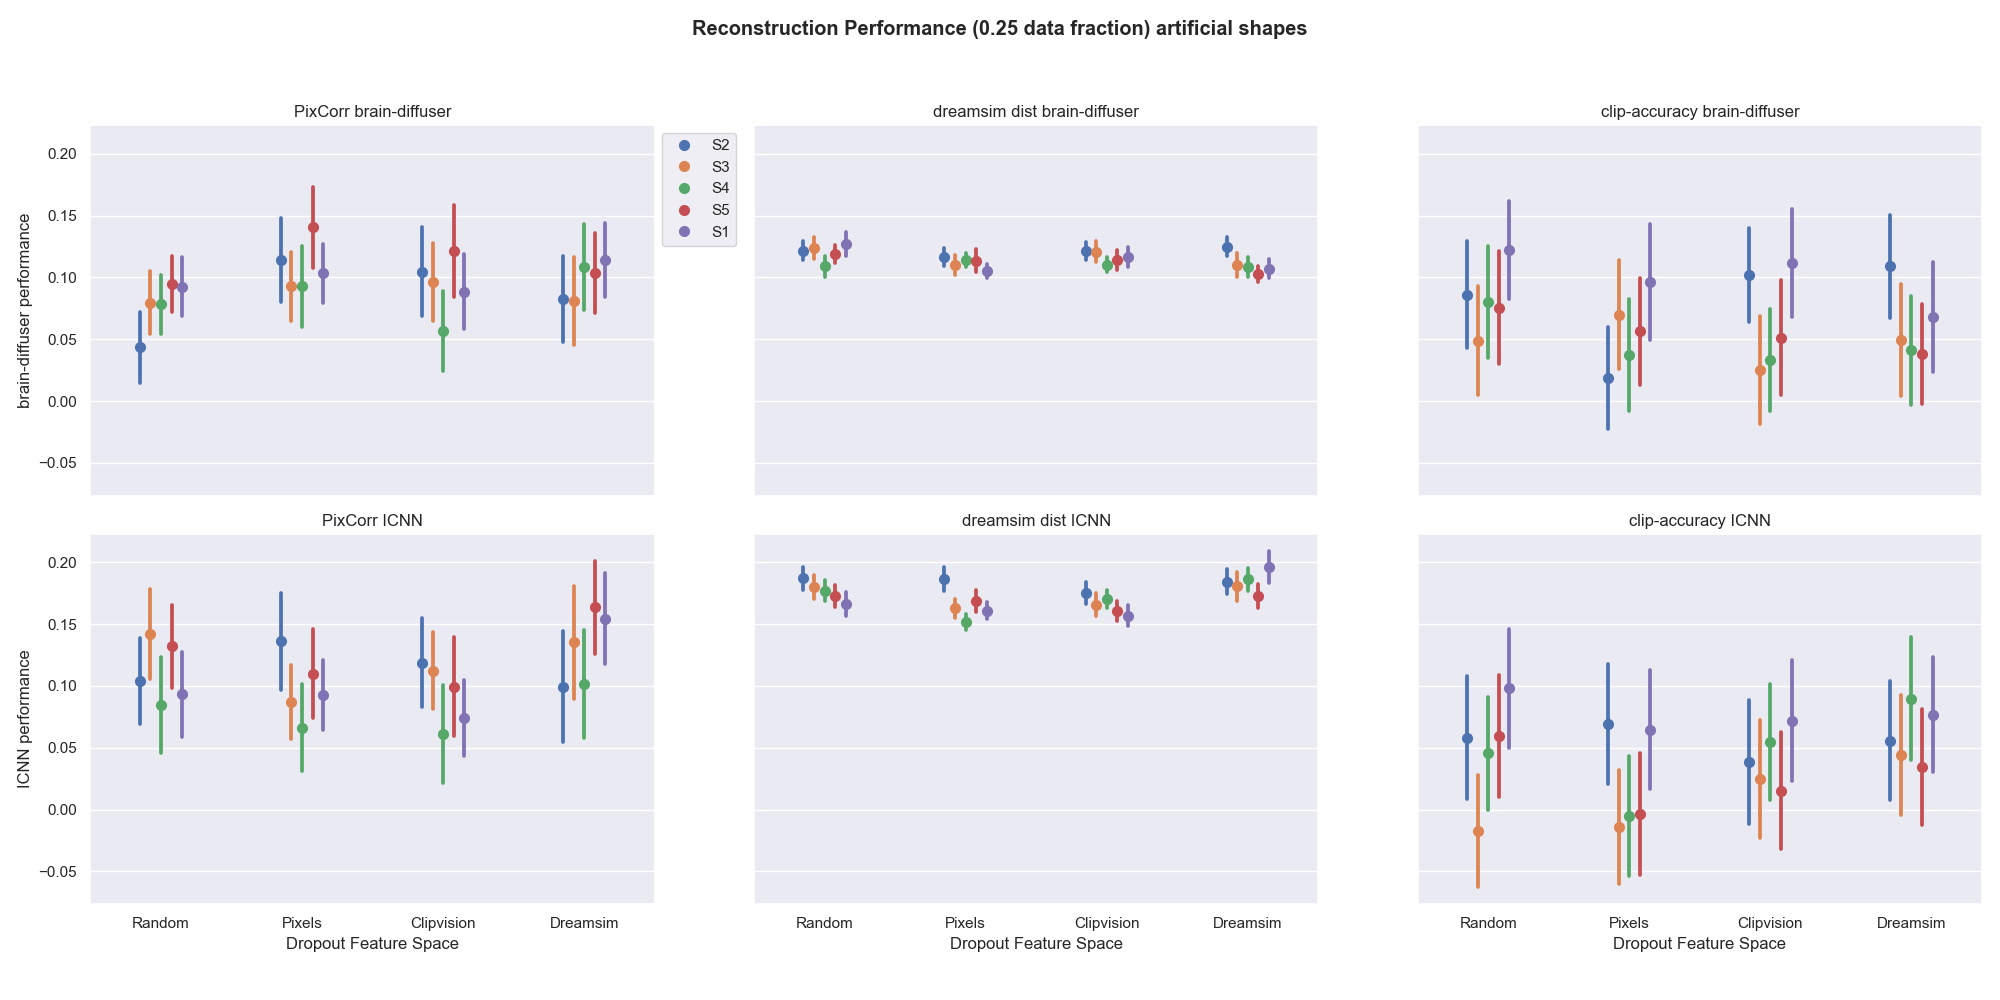
\includegraphics[width=1\textwidth]{plots/dropout_eval_reconstruction_art.png}
  \caption{Reconstruction Performance (0.25 data fraction) for Artificial Shapes}\label{fig:dropout_eval_reconstruction_art}
\end{figure}


Also for the artificial shapes in Figure~\ref{fig:dropout_eval_reconstruction_art}, the differences in reconstruction performance between the different feature spaces are small to not noticeable. For the brain diffuser it looks as if the pixel correlation with a dropout is slightly increased in the pixel subspace compared to the baseline. There are no visible differences in the other metrics. In the ICNN, the Dreamsim simulation appears slightly reduced in Pixels subspace and Clipvision subspace compared to the baseline. There are no visible differences in the Dreamsim subspace. 

As the quantitative results of the reconstruction performance suggest, a qualitative assessment of the differences in the reconstruction is difficult. The ICNN results for the natural test images are shown in Figure~\ref{fig:dropout_qual_eval_icnn_test} and for the artificial shapes in Figure~\ref{fig:dropout_qual_eval_icnn_art}. Differences in the quality of the reconstruction are difficult to determine; although it is clear that at least some reconstruction quality can be achieved in all conditions, the slight improvement of the feature spaces in contrast to the random baseline  seen in the quantitative results is not immediately apparent in the actual images. Likewise, for the artificial shapes in Figure~\ref{fig:dropout_qual_eval_icnn_art}, the slight degradation in the feature space results compared to the random sample is not directly apparent from the qualitative results. The quantitative results for the brain diffuser were even more ambiguous, so no major differences can be seen in the qualitative analysis of the images. The reconstructed images for the brain diffuser can be found in the appendix (Figure~\ref{fig:dropout_qual_eval_bd_test} for the natural test images and Figure~\ref{fig:dropout_qual_eval_bd_art} for the artificial shapes).


\begin{figure}[ht]
  \centering
  \includegraphics[width=1\textwidth]{plots/dropout_qual_eval_icnn_test.JPEG}
  \caption{A nice image}\label{fig:dropout_qual_eval_icnn_test}
\end{figure}

\begin{figure}[ht]
  \centering
  \includegraphics[width=1\textwidth]{plots/dropout_qual_eval_icnn_art.JPEG}
  \caption{A nice image}\label{fig:dropout_qual_eval_icnn_art}
\end{figure}



\subsection{Discussion}

- Man könnte den dropout noch stärker machen
- Durch die Evaluationskriterien wird sehr gut deutlich, DASS es einen Effekt gibt, aber nicht wie groß dieser ist und ob er wirklich bedeutsam ist
- Wir sind leider nur in der Lage das Subsampling top-down durchzuführen, also wenn ein großer schöner voller Datensatz zur Verfügung steht, besser wäre ein Bottom-Up approach, bei dem kein voller Datensatz von nöten ist. Wo man quasi ohne das gesamte Datenuniversum zu kennen die Qualität (bzw. Diversität) zweier subsampled Datasets untersuchen kann. 
- Man könnte auch weniger Cluster machen und dafür eins pro Cluster wählen, hat aber funkttioniert, also warum sollte ich.
- Brain-diffser hat Probleme
  -- Clipvision hat große Probleme bei den artificial Shapes überhaupt etwas zu lernen (siehe z.B. die Ergebnisse bei den random translatorn)
  -- Auch Cliptext ist dort nicht besonders gut. 
  -- Also versuchen wir im Folgenden genau an diesen beiden Stellschrauben was zu verändern um die Ergebnisse hier besser zu machen. 
- Category based dropout could be used instead (first, find the categories in the dataset)
